\chapter{Data Visualization}

\section{Line Plot \cite{wiki-line-chart}}\label{plot_line}
A line chart or line graph, also known as curve chart, is a type of chart that displays information as a series of data points called 'markers' connected by straight line segments. It is a basic type of chart common in many fields. It is similar to a scatter plot except that the measurement points are ordered (typically by their x-axis value) and joined with straight line segments. 


\begin{table}[H]
    \begin{minipage}{0.45\textwidth}
        \centering
        \begin{tabular}{|c|c|}
            \hline
            Elapsed Time ($s$) & Speed ($ms^{-1}$) \\ \hline
            0 & 0 \\ \hline
            1 & 3 \\ \hline
            2 & 7 \\ \hline
            3 & 12 \\ \hline
            4 & 18 \\ \hline
            5 & 30 \\ \hline
            6 & 45.6 \\ \hline
        \end{tabular}
        \caption{Data: Line Plot}
    \end{minipage}
    \hfill
    \begin{minipage}{0.45\textwidth}
        \begin{figure}[H]
            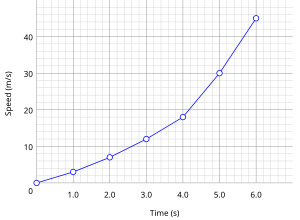
\includegraphics[width=\linewidth]{Pictures/data/data_line_chart.jpg}
            \caption{Graph: Line Plot}
        \end{figure}
    \end{minipage}
\end{table}


\section{Bar Graph \cite{wiki-bar-chart}}\label{graph_bar}
A bar chart or bar graph is a chart or graph that presents categorical data with rectangular bars with heights or lengths proportional to the values that they represent. The bars can be plotted vertically or horizontally. A vertical bar chart is sometimes called a \textbf{column chart}\indexlabel{column chart}.

\vspace{-1cm}

\begin{center}
    \begin{figure}
        \centering
        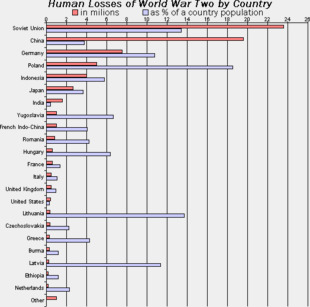
\includegraphics[height=5.6cm]{Pictures/data/data_graph_bar.jpg}
        \caption{Graph: Bar Graph}
    \end{figure}
\end{center}


\section{Histogram \cite{ism-2, wiki-histogram}}\label{histogram}
\subsection{Constructing a Histogram for Discrete Data}
\begin{enumerate}
    \item determine the frequency and relative frequency of each x value
    \item mark possible x values on a horizontal scale
    \item Above each x value, draw a rectangle whose height is the relative frequency (or alternatively, the frequency) of that value
\end{enumerate}

\subsection{Constructing a Histogram for Continuous Data: Equal Class Widths}
\begin{enumerate}
    \item Determine the frequency and relative frequency for each class.
    \item Mark the class boundaries on a horizontal measurement axis.
    \item Above each class interval, draw a rectangle whose height is the corresponding relative frequency (or frequency).
\end{enumerate}

\subsection{Constructing a Histogram for Continuous Data: Unequal Class Widths}
\begin{enumerate}
    \item After determining frequencies and relative frequencies, calculate the height of each rectangle using the formula:
    \begin{equation}
        (rectangle\_height) = (relative\_frequency\_of\_the\_class) / (class\_width)
    \end{equation}
    \item The resulting rectangle heights are usually called \textbf{densities}\indexlabel{densities (histogram)}, and the vertical scale is the density scale. 
    \item This prescription will also work when class widths are equal. 
    \item the area of each rectangle is proportional to the relative frequency of the value
\end{enumerate}

\begin{table}[H]
    \begin{minipage}{0.45\textwidth}
        \centering
        \begin{tabular}{|c|c|}
            \hline
            Bin/Interval & Count/Frequency \\ \hline
            -3.5 to -2.51 & 9 \\ \hline
            -2.5 to -1.51 & 32 \\ \hline
            -1.5 to -0.51 & 109 \\ \hline
            -0.5 to 0.49 & 180 \\ \hline
            0.5 to 1.49 & 132 \\ \hline
            1.5 to 2.49 & 34 \\ \hline
            2.5 to 3.49 & 4 \\ \hline
        \end{tabular}
        \caption{Data: Histogram}
    \end{minipage}
    \hfill
    \begin{minipage}{0.45\textwidth}
        \begin{figure}[H]
            \centering
            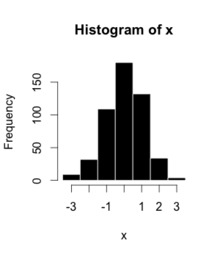
\includegraphics[height=5cm]{Pictures/data/data_histogram.jpg}
            \caption{Graph: Histogram}
        \end{figure}
    \end{minipage}
\end{table}


\section{Stem-and-Leaf Displays \cite{ism-2,wiki-Stem-and-leaf_display}}\label{Stem-and-Leaf Displays}
\begin{enumerate}
    \item Consider a numerical data set x1, .., xn for which each xi consists of at least two digits. 
    \item A quick way to obtain an informative visual representation of the data set is to construct a stem-and-leaf display.
    \item A stem-and-leaf display conveys information about the following aspects of the data:
    \begin{enumerate}
        \item identification of a typical or representative value
        \item extent of spread about the typical value
        \item presence of any gaps in the data
        \item extent of symmetry in the distribution of values
        \item number and location of peaks
        \item presence of any outlying values
    \end{enumerate}
\end{enumerate}
\subsection{Constructing a Stem-and-Leaf Display}
\begin{enumerate}
    \item Select one or more leading digits for the stem values. The trailing digits become the leaves
    \item List possible stem values in a vertical column.
    \item Record the leaf for each observation beside the corresponding stem value
    \item Indicate the units for stems and leaves someplace in the display
\end{enumerate}

\section{Dotplots \cite{wiki-dotplot,ism-2}}\label{dotplots}
\begin{enumerate}
    \item A dotplot is an attractive summary of numerical data when the data set is reasonably small or there are relatively few distinct data values. 
    \item Each observation is represented by a dot above the corresponding location on a horizontal measurement scale. 
    \item When a value occurs more than once, there is a dot for each occurrence, and these dots are stacked vertically
    \item A dotplot gives information about location, spread, extremes, and gaps
\end{enumerate}

\begin{figure}
    \centering
    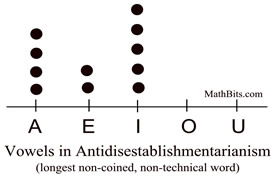
\includegraphics[height=3cm]{Pictures/data/data_dotplot.jpg}
    \caption{Graph: Dotplot}
\end{figure}

\section{Quantile-Quantile Plot \cite{wiki-q-q-plot}}\label{Quantile-Quantile Plot}
A Q–Q plot (quantile–quantile plot) is a probability plot, a graphical method for comparing two probability distributions by plotting their quantiles against each other. A point (x, y) on the plot corresponds to one of the quantiles of the second distribution (y-coordinate) plotted against the same quantile of the first distribution (x-coordinate). This defines a parametric curve where the parameter is the index of the quantile interval.

\begin{table}[H]
    \begin{minipage}{0.45\textwidth}
        \begin{figure}[H]
            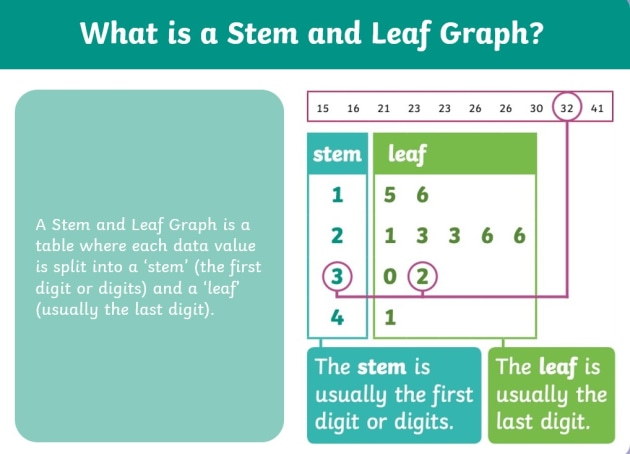
\includegraphics[height=5cm]{Pictures/data/data_stem-and-leaf-plot.jpg}
            \caption{Graph: Stem \& Leaf Plot}
        \end{figure}
    \end{minipage}
    \hfill
    \begin{minipage}{0.45\textwidth}
        \begin{figure}[H]
            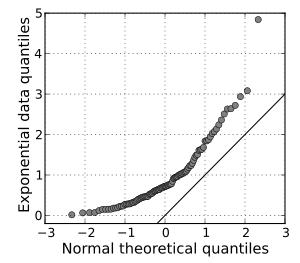
\includegraphics[height=5cm]{Pictures/data/data_q_q_plot.png}
            \caption{Graph: Quantile–Quantile (Q–Q) plot}
        \end{figure}
    \end{minipage}
\end{table}


\section{Box and Whisker plots (aka Box Plot)}\label{Box and Whisker plots (aka Box Plot)}
A box plot or boxplot is a method for demonstrating graphically the locality, spread and skewness groups of numerical data through their quartiles. In addition to the box on a box plot, there can be lines (which are called whiskers) extending from the box indicating variability outside the upper and lower quartiles, thus, the plot is also called the box-and-whisker plot and the box-and-whisker diagram. Outliers that differ significantly from the rest of the dataset may be plotted as individual points beyond the whiskers on the box-plot. Box plots are non-parametric: they display variation in samples of a statistical population without making any assumptions of the underlying statistical distribution (though Tukey's boxplot assumes symmetry for the whiskers and normality for their length). The spacings in each subsection of the box-plot indicate the degree of dispersion (spread) and skewness of the data, which are usually described using the five-number summary. In addition, the box-plot allows one to visually estimate various L-estimators, notably the interquartile range, midhinge, range, mid-range, and trimean. Box plots can be drawn either horizontally or vertically.

\begin{enumerate}
    \item features:
    \begin{enumerate}
        \item center
        \item spread
        \item the extent and nature of any departure from symmetry
        \item identification of “outliers”
    \end{enumerate}
\end{enumerate}

\subsection{Steps to build Box plot}
\begin{enumerate}
    \item Order the n observations from smallest to largest and separate the smallest half from the largest half; the median is included in both halves if n is odd.
    \item Then the lower fourth (1st quartile) is the median of the smallest half and the upper fourth (3rd quartile) is the median of the largest half.
    \item A measure of spread that is resistant to outliers is the fourth spread (aka IQR) fs, given by fs = upper fourth - lower fourth
    \item Any observation farther than 1.5fs from the closest fourth is an outlier
    \item An outlier is extreme if it is more than 3fs from the nearest fourth, and it is mild otherwise.
    \item draw a horizontal measurement scale
    \item place a rectangle above this axis; the left edge of the rectangle is at the lower fourth, and the right edge is at the upper fourth (box width = fs)
    \item Place a vertical line segment or some other symbol inside the rectangle at the location of the median; the position of the median symbol relative to the two edges conveys information about skewness in the middle 50% of the data
    \item draw “whiskers” out from either end of the rectangle to the smallest and largest observations that are not outliers
    \item Each mild outlier is represented by a closed circle and each extreme outlier by an open circle
\end{enumerate}

\begin{figure}[H]
    \centering
    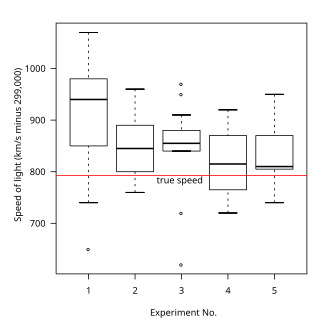
\includegraphics[height=6cm]{Pictures/data/data_box-plot.jpg}
    \caption{Graph: Box Plot}
\end{figure}































